\documentclass[man,floatsintext]{apa6}
\usepackage{lmodern}
\usepackage{amssymb,amsmath}
\usepackage{ifxetex,ifluatex}
\usepackage{fixltx2e} % provides \textsubscript
\ifnum 0\ifxetex 1\fi\ifluatex 1\fi=0 % if pdftex
  \usepackage[T1]{fontenc}
  \usepackage[utf8]{inputenc}
\else % if luatex or xelatex
  \ifxetex
    \usepackage{mathspec}
  \else
    \usepackage{fontspec}
  \fi
  \defaultfontfeatures{Ligatures=TeX,Scale=MatchLowercase}
\fi
% use upquote if available, for straight quotes in verbatim environments
\IfFileExists{upquote.sty}{\usepackage{upquote}}{}
% use microtype if available
\IfFileExists{microtype.sty}{%
\usepackage{microtype}
\UseMicrotypeSet[protrusion]{basicmath} % disable protrusion for tt fonts
}{}
\usepackage{hyperref}
\hypersetup{unicode=true,
            pdftitle={papaja: Prepare Computationally Reproducible APA Journal Articles with R Markdown},
            pdfauthor={Frederik Aust~\& Marius Barth},
            pdfkeywords={computational reproducibility, method robustness, repeatability, dynamic
documents},
            pdfborder={0 0 0},
            breaklinks=true}
\urlstyle{same}  % don't use monospace font for urls
\usepackage{color}
\usepackage{fancyvrb}
\newcommand{\VerbBar}{|}
\newcommand{\VERB}{\Verb[commandchars=\\\{\}]}
\DefineVerbatimEnvironment{Highlighting}{Verbatim}{commandchars=\\\{\}}
% Add ',fontsize=\small' for more characters per line
\usepackage{framed}
\definecolor{shadecolor}{RGB}{248,248,248}
\newenvironment{Shaded}{\begin{snugshade}}{\end{snugshade}}
\newcommand{\KeywordTok}[1]{\textcolor[rgb]{0.13,0.29,0.53}{\textbf{#1}}}
\newcommand{\DataTypeTok}[1]{\textcolor[rgb]{0.13,0.29,0.53}{#1}}
\newcommand{\DecValTok}[1]{\textcolor[rgb]{0.00,0.00,0.81}{#1}}
\newcommand{\BaseNTok}[1]{\textcolor[rgb]{0.00,0.00,0.81}{#1}}
\newcommand{\FloatTok}[1]{\textcolor[rgb]{0.00,0.00,0.81}{#1}}
\newcommand{\ConstantTok}[1]{\textcolor[rgb]{0.00,0.00,0.00}{#1}}
\newcommand{\CharTok}[1]{\textcolor[rgb]{0.31,0.60,0.02}{#1}}
\newcommand{\SpecialCharTok}[1]{\textcolor[rgb]{0.00,0.00,0.00}{#1}}
\newcommand{\StringTok}[1]{\textcolor[rgb]{0.31,0.60,0.02}{#1}}
\newcommand{\VerbatimStringTok}[1]{\textcolor[rgb]{0.31,0.60,0.02}{#1}}
\newcommand{\SpecialStringTok}[1]{\textcolor[rgb]{0.31,0.60,0.02}{#1}}
\newcommand{\ImportTok}[1]{#1}
\newcommand{\CommentTok}[1]{\textcolor[rgb]{0.56,0.35,0.01}{\textit{#1}}}
\newcommand{\DocumentationTok}[1]{\textcolor[rgb]{0.56,0.35,0.01}{\textbf{\textit{#1}}}}
\newcommand{\AnnotationTok}[1]{\textcolor[rgb]{0.56,0.35,0.01}{\textbf{\textit{#1}}}}
\newcommand{\CommentVarTok}[1]{\textcolor[rgb]{0.56,0.35,0.01}{\textbf{\textit{#1}}}}
\newcommand{\OtherTok}[1]{\textcolor[rgb]{0.56,0.35,0.01}{#1}}
\newcommand{\FunctionTok}[1]{\textcolor[rgb]{0.00,0.00,0.00}{#1}}
\newcommand{\VariableTok}[1]{\textcolor[rgb]{0.00,0.00,0.00}{#1}}
\newcommand{\ControlFlowTok}[1]{\textcolor[rgb]{0.13,0.29,0.53}{\textbf{#1}}}
\newcommand{\OperatorTok}[1]{\textcolor[rgb]{0.81,0.36,0.00}{\textbf{#1}}}
\newcommand{\BuiltInTok}[1]{#1}
\newcommand{\ExtensionTok}[1]{#1}
\newcommand{\PreprocessorTok}[1]{\textcolor[rgb]{0.56,0.35,0.01}{\textit{#1}}}
\newcommand{\AttributeTok}[1]{\textcolor[rgb]{0.77,0.63,0.00}{#1}}
\newcommand{\RegionMarkerTok}[1]{#1}
\newcommand{\InformationTok}[1]{\textcolor[rgb]{0.56,0.35,0.01}{\textbf{\textit{#1}}}}
\newcommand{\WarningTok}[1]{\textcolor[rgb]{0.56,0.35,0.01}{\textbf{\textit{#1}}}}
\newcommand{\AlertTok}[1]{\textcolor[rgb]{0.94,0.16,0.16}{#1}}
\newcommand{\ErrorTok}[1]{\textcolor[rgb]{0.64,0.00,0.00}{\textbf{#1}}}
\newcommand{\NormalTok}[1]{#1}
\usepackage{longtable,booktabs}
\usepackage{graphicx,grffile}
\makeatletter
\def\maxwidth{\ifdim\Gin@nat@width>\linewidth\linewidth\else\Gin@nat@width\fi}
\def\maxheight{\ifdim\Gin@nat@height>\textheight\textheight\else\Gin@nat@height\fi}
\makeatother
% Scale images if necessary, so that they will not overflow the page
% margins by default, and it is still possible to overwrite the defaults
% using explicit options in \includegraphics[width, height, ...]{}
\setkeys{Gin}{width=\maxwidth,height=\maxheight,keepaspectratio}
\IfFileExists{parskip.sty}{%
\usepackage{parskip}
}{% else
\setlength{\parindent}{0pt}
\setlength{\parskip}{6pt plus 2pt minus 1pt}
}
\setlength{\emergencystretch}{3em}  % prevent overfull lines
\providecommand{\tightlist}{%
  \setlength{\itemsep}{0pt}\setlength{\parskip}{0pt}}
\setcounter{secnumdepth}{0}
% Redefines (sub)paragraphs to behave more like sections
\ifx\paragraph\undefined\else
\let\oldparagraph\paragraph
\renewcommand{\paragraph}[1]{\oldparagraph{#1}\mbox{}}
\fi
\ifx\subparagraph\undefined\else
\let\oldsubparagraph\subparagraph
\renewcommand{\subparagraph}[1]{\oldsubparagraph{#1}\mbox{}}
\fi

%%% Use protect on footnotes to avoid problems with footnotes in titles
\let\rmarkdownfootnote\footnote%
\def\footnote{\protect\rmarkdownfootnote}


  \title{papaja: Prepare Computationally Reproducible APA Journal Articles with R
Markdown}
    \author{Frederik Aust\textsuperscript{}~\& Marius Barth\textsuperscript{}}
    \date{}
  
\shorttitle{papaja}
\affiliation{
\vspace{0.5cm}
\textsuperscript{} University of Cologne}
\keywords{computational reproducibility, method robustness, repeatability, dynamic documents\newline\indent Word count: }
\usepackage{csquotes}
\usepackage{upgreek}
\captionsetup{font=singlespacing,justification=justified}

\usepackage{longtable}
\usepackage{lscape}
\usepackage{multirow}
\usepackage{tabularx}
\usepackage[flushleft]{threeparttable}
\usepackage{threeparttablex}

\newenvironment{lltable}{\begin{landscape}\begin{center}\begin{ThreePartTable}}{\end{ThreePartTable}\end{center}\end{landscape}}

\makeatletter
\newcommand\LastLTentrywidth{1em}
\newlength\longtablewidth
\setlength{\longtablewidth}{1in}
\newcommand{\getlongtablewidth}{\begingroup \ifcsname LT@\roman{LT@tables}\endcsname \global\longtablewidth=0pt \renewcommand{\LT@entry}[2]{\global\advance\longtablewidth by ##2\relax\gdef\LastLTentrywidth{##2}}\@nameuse{LT@\roman{LT@tables}} \fi \endgroup}


\usepackage{lineno}

\linenumbers

\authornote{Frederik Aust and Marius Barth, Department
Psychology, University of Cologne, Germany.

We thank everyone who contributed to the development of papaja by
suggesting enhancements, reporting bugs, and asking questions.

Correspondence concerning this article should be addressed to Frederik
Aust, Herbert-Lewin-Str. 2, 50931 Cologne, Germany. E-mail:
\href{mailto:frederik.aust@uni-koeln.de}{\nolinkurl{frederik.aust@uni-koeln.de}}}
\note{This manuscript is an early draft published primarily to
elicit feedback and obtain a DOI that can be used to cite and thus
credit papaja in published articles. }
\abstract{
Computational reproduciblity is the ability to reproduce the results of
a analytic or computational procedure when given the same input data
(and analysis scripts). Recent research has demonstrated empirically
that, given the original data, results in scientific reports from a
variety of disciplines are often difficult and sometimes impossible to
reproduce. Baring in mind that computational reproducibility is a basic
requirement for intersubjective verifiability it must be considered a
minimum requirement to consider scientific claims. The difficulty to
reproduce results in peer-reviewed scientific journal articles,
therefore, highlight a serious problem with the widespread
copy-and-paste approach to scientific reporting. We argue that dynamic
documents are a more reliable approach to authoring scientific reports:
By fusing manuscript and analysis scripts dynamic documents help to
ensure the computational reporducibility of reported results. We
furthermore introduce the R package papaja that is designed to author
APA-style manuscripts in R Markdown and facilitates the standardized
reporting of analyses common in psychological research.



}

\usepackage{amsthm}
\newtheorem{theorem}{Theorem}[section]
\newtheorem{lemma}{Lemma}[section]
\theoremstyle{definition}
\newtheorem{definition}{Definition}[section]
\newtheorem{corollary}{Corollary}[section]
\newtheorem{proposition}{Proposition}[section]
\theoremstyle{definition}
\newtheorem{example}{Example}[section]
\theoremstyle{definition}
\newtheorem{exercise}{Exercise}[section]
\theoremstyle{remark}
\newtheorem*{remark}{Remark}
\newtheorem*{solution}{Solution}
\begin{document}
\maketitle

The dominant approach to writing scientific reports in psychology is the
use of common word processors such as Microsoft Word or Libre Office. To
implement the commonly requested APA manuscript style\footnote{APA style
  is one of the major style regimes in academia concerned with written
  scientific communication and is defined in the \emph{Publication
  Manual of the American Psychological Association} (APA; American
  Psychological Association, 2010). Research in psychology and many
  fields other, including other social sciences, medicine, and public
  health is reported in APA style.}, authors may use document templates
set up page margins, line spacing, fonts, and related aspects of the
manuscript. The format of citations and references can be automated by
using references managers that integrate with the word processor. These
forms of automation facilitate the implementation of APA style and
reduce the likelihood of formatting errors. In contrast to manuscript
styling, reporting of results is typically not automated. Results of
analyses are copied from the output of the analysis software and pasted
into the word processor. We will, therefore, refer to this as
\emph{copy-and-paste reporting}. Error-free reporting of results is
arguably more important for a cummulative science than the manuscript
style. Nonetheless, copy-and-paste reporting employs fault-preventing
autmation only to ensure correct manuscript styling but not to ensure
correct reporting or results.

Recent research has demonstrated empirically that, given the original
data, results in scientific reports from a variety of disciplines are
often difficult and sometimes impossible to reproduce {[}citations
needed{]}. This nonreproducability of results in peer-reviewed
scientific journal articles indicates a serious problem with
copy-and-paste reporting. In the following, we argue that dynamic
documents are a less error-prone approach to authoring scientific
reports: By fusing manuscript and analysis scripts dynamic documents
help to ensure the computational reporducibility of reported results. We
introduce the R package \texttt{papaja} that is designed to author
APA-style manuscripts in R Markdown and facilitates the standardized
reporting of analyses common in psychological research.

\section{Computation reproducibility}\label{computation-reproducibility}

\ldots{}

Thus, the term reproducibility here means that given a dataset and
analysis script any analyst obtains the same statistical results
(Asendorpf et al., 2013; Cacioppo, Kaplan, Krosnick, Olds, \& Dean,
2015).

The importance of reproducibility was pinpointed by the U.S. National
Science Foundation subcommittee on replicability in science:

\begin{quote}
Reproducibility is a minimum necessary condition for a finding to be
believable and informative. (p.~4, Cacioppo et al., 2015)
\end{quote}

\begin{quote}
Good statistical practice is fundamentally based on transparent
assumptions, reproducible results, and valid interpretations.
\end{quote}

\begin{quote}
The ethical statistician {[}\ldots{}{]} strives to promote transparency
in design, execution, and reporting or presenting of all analyses
\end{quote}

\begin{quote}
Makes documentation suitable for replicate analyses, metadata studies,
and other research by qualified investigators.
\end{quote}

\url{http://www.amstat.org/asa/files/pdfs/EthicalGuidelines.pdf}

\enquote{an article about a computational result is advertising, not
scholarship. The actual scholarship is the full software environment,
code and data, that produced the result.} - Buckheit \& Donoho, 1995

(Elsevier executable paper challenge: 10.1016/j.procs.2011.04.064)

Donoho, D. L., Maleki, A., Rahman, I. U., Shahram, M. \& Stodden, V.
Reproducible research in computational harmonic analysis. Comput. Sci.
Eng. 11, 8--18 (2009). Donoho and fellow researchers have been at the
forefront of reproducibility for many years; this a

\begin{enumerate}
\def\labelenumi{\arabic{enumi}.}
\tightlist
\item
  Generalizability (e.g., Baribault et al., 2017; Brandt et al., 2014)
\item
  Replicability (e.g., Open Science Collaboration, 2015; Simons, 2014)
\item
  Analytical robustness (e.g., Silberzahn et al., 2017; Simonsohn,
  Simmons, \& Nelson, 2015; Steegen, Tuerlinckx, Gelman, \& Vanpaemel,
  2016)
\item
  Computational reproducibility (e.g., Peng, 2011; Rokem, Marwick, \&
  Staneva, 2017; Stodden, 2015)
\end{enumerate}

But see, for example, Plesser (2018)

U.S. National Science Foundation (NSF) subcommittee on replicability in
science:

\begin{quote}
{[}Computational{]} Reproducibility is a .highlight{[}minimum necessary
condition for a finding to be believable and informative{]}. (p.~4,
Cacioppo, Kaplan, Krosnick, Olds, \& Dean, 2015)
\end{quote}

~

\begin{quote}
It is .highlight{[}scientifically and ethically imperative{]} that the
results of statistical analysis {[}\ldots{}{]} be computationally
reproducible (p.~138, Liu \& Pounds, 2014)
\end{quote}

\section{Prevalence of computational
nonreproducibility}\label{prevalence-of-computational-nonreproducibility}

--\textgreater{}

\section{Reproducible scientific
reports}\label{reproducible-scientific-reports}

Dynamic scientific reports fuse prose and simulation or analysis scripts
(Gandrud, 2013; Xie, 2015). Each time a dynamic document is compiled,
the scripts are executed anew and the results---statistics, tables, and
figures---are recreated and inserted into the document. Thereby dynamic
documents allow automated reporting of results, which is currently not
possible with the prevalent use of Microsoft Word or Libre Office.
Importantly, dynamic documents ensure that the results reported in the
manuscript are free of rounding or transcription errors and correspond
to the performed analyses. This is the reason why dynamic scientific
reports are commonly referred to as reproducible scientific reports or
reproducible reports.

\hypertarget{document-compilation}{\subsubsection{Document
compilation}\label{document-compilation}}

It is important to note that \texttt{papaja} builds on several existing
R packages, which in turn build on other software, to compile the final
document. This layered software design grants the package its
capabilities but it comes at a cost: When compilation of a
\texttt{papaja}-document throws an error it may not be immediately
obvious to an inexperienced user, which part of the process failed. We,
thus, provide an overview of the compilation process and the software
involved.

As detailed in the {[}R Markdown components{]} section, an R Markdown
document consists of three components: A YAML front matter that contains
document meta data, prose written in markdown (and optionally LaTeX)
syntax, and R code in so-called \emph{code chunks}.

Additionally, the R code contained in an R Markdown document usually
accesses data that are either stored in a file on the computers hard
drive or a database on the local network or internet. When the document
is compiled either by calling \texttt{rmarkdown::render()} or by
clicking the Knit-button in RStudio, the YAML front matter is parsed.
Errors during this processing step are usually due to erroneous YAML
syntax and start with
\texttt{Error\ in\ yaml::yaml.load(enc2utf8(string),\ ...)\ :}. Next,
the R code inside the R Markdown document is executed sequentially from
top to bottom of the document and the resulting output is inserted into
the document in markdown syntax. Any figures that are generated during
the execution of the R code are stored to the hard drive and embedded
into the markdown document. The R code is executed in a new R session
with an empty workspace, no attached packages, and with the working
directory set to the path of the R Markdown file. If any portion of the
R code throws an error the compilation is aborted. In RStudio the
debugger will point to the first line of the R code chunk that threw the
error---not the exact line responsible for the error---and report the
error message. R error messages usually start with \texttt{Error:}, for
example,
\texttt{Error:\ Object\ \textquotesingle{}experiment\_data\textquotesingle{}\ not\ found.}








\begin{figure}

{\centering 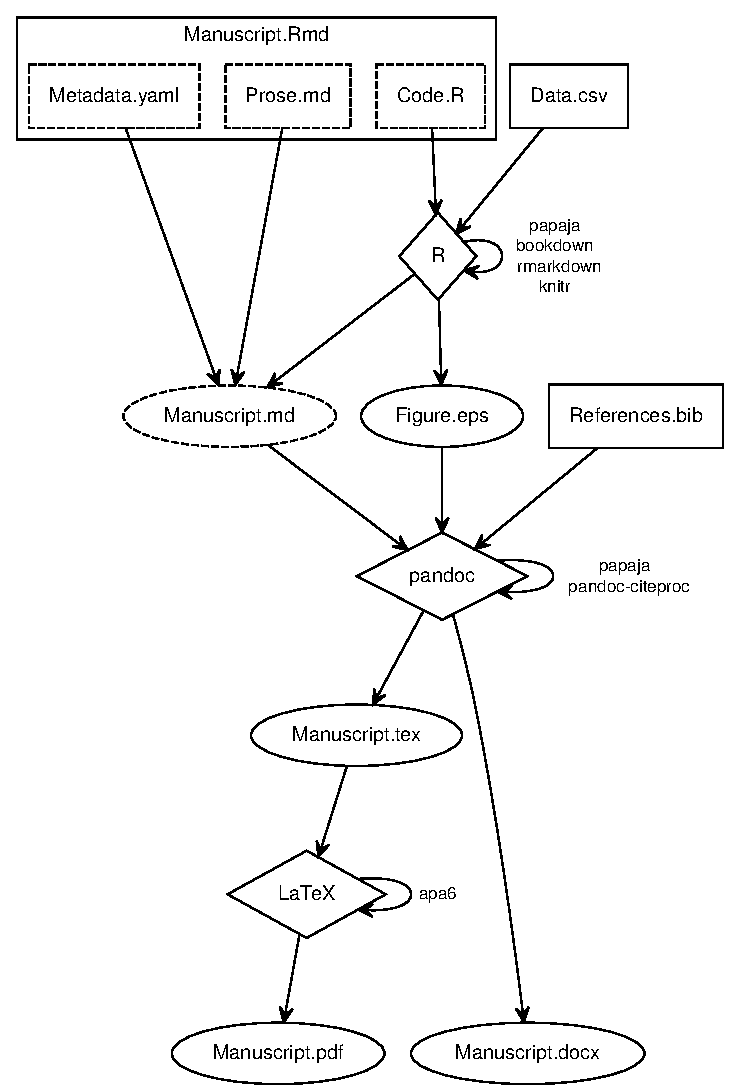
\includegraphics{paper_files/figure-latex/compilation-process-diagram} 

}

\caption{Process diagram illustrating the
compilation of reproducible reports written with \texttt{papaja}. Boxes
represent input files, diamonds represent compiling software, and ovals
represent output files. Dashed components are either implicit
(components of R Markdown files) or by default deleted after the
compilation and, thus, invisible to the user.}\label{fig:compilation-process-diagram}
\end{figure}

After the R code has been executed the \texttt{bookdown} document format
\texttt{pdf\_document2()} or \texttt{word\_document2()}, respectively,
provides functions that enable the cross-referencing syntax
\texttt{\textbackslash{}@ref()} described in the
\protect\hyperlink{cross-referencing}{Cross-referencing} section.
Incorrect use of the cross-referencing syntax typically does not
interfere with the document compilation but is apparent from missing or
incorrect cross-references in the compiled document, e.g.~instead of a
figure number the document may contain the figure handle such as
\texttt{\label{fig:my-figure}}. The result of this processing step is a pure
markdown document containing only a YAML header, prose in markdown (and
optionally LaTeX) syntax and rendered images in PDF, EPS, PNG, and TIFF
formats at 300 dpi as set by \texttt{apa6\_pdf()} or
\texttt{apa6\_word()}, respectively.

The markdown document, images and an optional BiB(La)TeX file that
contains bibliographic information are the input to the next processing
step. \texttt{rmarkdown::render()} assembles a system call to pandoc
that is supplemented by \texttt{papaja} to include a call to an
additional filter and can be further customized by the user. pandoc
parses the contents of the markdown file and translates it into an
abstract syntax tree (AST). The \texttt{pandoc-citeproc} filter is than
applied to the AST to replace the citation markup by the citation text
and insert a reference section. As detailed in the
\protect\hyperlink{citations}{Citations} section,
\texttt{pandoc-citeproc} relies on the
\href{http://citationstyles.org/}{citation styles language} (CSL), an
XML-based specification of citation and bibliography formatting rules.
Unfortunately, CSL does not support in-text citations. To overcome this
limitation, \texttt{pandoc-citeproc} provides a separate syntax for
in-text citations, which is based on the same CSL style. As a result the
CSL APA6 style uses ampersands for all citations, including in-text
citations, defying the APA citation style. That is why \texttt{papaja}
provides an additional R-based filter that is applied to the AST to
replace ampersands in in-text citations with the word \emph{and}.

After all filters have been applied to the AST pandoc converts the
document into the target output format, that is, PDF or DOCX. To create
DOCX-documents \texttt{papaja} provides a reference DOCX-file containing
page setup and style definitions that pandoc uses to create the
manuscript file. That is, pandoc translates the AST directly to the
office open XML format. To create PDF-documents pandoc in turn relies on
LaTeX, that is, pandoc translates the AST to a TeX-file based on a
template provided by \texttt{papaja}. This template invokes the
\texttt{apa6} LaTeX document class {[}@???{]} and loads several
additional LaTeX packages. pandoc then generates a system call to LaTeX
to render the PDF document. During this processing step, that is,
following the pandoc system calls, errors are due to failures of LaTeX
to compile the TeX-file and usually start with \texttt{!}, for example,
\texttt{!\ Undefined\ control\ sequence.} or
\texttt{!\ Missing\ \$\ inserted}.

\begin{itemize}
\tightlist
\item
  YAML front matter is read

  \begin{itemize}
  \tightlist
  \item
    \texttt{Error\ in\ yaml::yaml.load(enc2utf8(string),\ ...)\ :}
  \end{itemize}
\item
  R code is executed

  \begin{itemize}
  \tightlist
  \item
    \texttt{Error:\ Object\ \textquotesingle{}experiment\_data\textquotesingle{}\ not\ found.}
  \item
    Gives first line of erroneous R code chunk
  \end{itemize}
\item
  \texttt{bookdown} adds cross- and text-references

  \begin{itemize}
  \tightlist
  \item
    No error messages; look for \texttt{\label{fig:chunk-name}} in text
  \item
    Don't use \texttt{\_} in chunk names!
  \end{itemize}
\item
  \texttt{pandoc} and \texttt{pandoc-citeproc} convert Markdown

  \begin{itemize}
  \tightlist
  \item
    \texttt{Error:\ pandoc\ document\ conversion\ failed\ with\ error\ 1}
  \item
    \texttt{pandoc-citeproc:\ Cannot\ decode\ byte\ \textquotesingle{}\textbackslash{}xfc\textquotesingle{}}
  \item
    \texttt{pandoc-citeproc:\ reference\ XYZ\ not\ found},shows up as
    \textbf{???} in text
  \end{itemize}
\item
  LaTeX creates a PDF

  \begin{itemize}
  \tightlist
  \item
    \texttt{!\ Missing\ \$\ inserted}
  \end{itemize}
\end{itemize}

\subsubsection{Software requirements}\label{software-requirements}

To use \texttt{papaja} you need to make sure the following software is
installed on your computer:

\begin{enumerate}
\def\labelenumi{\arabic{enumi}.}
\tightlist
\item
  \textbf{\href{http://www.r-project.org/}{R} 2.11.1 or later}
\item
  \textbf{\href{http://johnmacfarlane.net/pandoc/}{pandoc} 1.19 or
  later}; if you work with \href{http://www.rstudio.com/}{RStudio}
  (1.1.453 or later) pandoc should already be installed, otherwise
  install pandoc using the
  \href{https://github.com/rstudio/rmarkdown/blob/master/PANDOC.md}{instructions
  for your operating system}
\end{enumerate}

If you want to create PDF- in addition to DOCX-files you need

\begin{enumerate}
\def\labelenumi{\arabic{enumi}.}
\setcounter{enumi}{2}
\tightlist
\item
  \textbf{\href{http://de.wikipedia.org/wiki/TeX}{TeX} 2013 or later}.
  Try \href{http://miktex.org/}{MikTeX} for Windows,
  \href{https://tug.org/mactex/}{MacTeX} for Mac, or
  \href{http://www.tug.org/texlive/}{TeX Live} for Linux.
\end{enumerate}

\texttt{papaja} requires LaTeX packages that are not part of the basic
TeX installations.

\section{Document structure}\label{document-structure}

\subsection{Body}\label{body}

The body of R Markdown documents consists of prose written in Markdown
interspersed with R code.

\subsubsection{Markdown}\label{markdown}

A general principle in typesetting is to separate content and style.
Separation is commonly achieved through the use of a markup language,
which is a system of document annotations. These annotations declare
portions of text as, for example, title, section headings, or list items
but, crucially, they are agnostic to what this means visually (e.g.,
\texttt{**text**} instead of \textbf{text}). Separation of content and
style is useful because it enables swift changes to an entire documents'
style or structure and facilitates applying a common style across
multiple documents. Microsoft Word implements this strategy in their
so-called \emph{styles}, which are collections of formatting
instructions that can be assigned to portions of the text.

\texttt{papaja} uses the
\href{http://en.wikipedia.org/wiki/Markdown}{Markdown} syntax to
separate content and style. Markdown was desigend to be an easy-to-read
and -write formatting syntax. The key design goal was to create a syntax
that is readable as-is. The following is an excerpt from the APA example
manuscript written in Markdown.

Without any prior knowledge of Markdown it should be easy to guess what
most of this syntax does: \texttt{\#} and \texttt{\#\#} denote first and
second order section headings (and so on), \texttt{\textless{}!-\/-} and
\texttt{-\/-\textgreater{}} surround comments that will not be displayed
in the rendered document, and \texttt{{[}\^{}p{]}} adds a reference to a
footnote that is written out following \texttt{{[}\^{}p{]}:}. The
equations surrounded by \texttt{\$} may be somewhat less intuitive. In R
Markdown, equations are written in LaTeX's powerful
\href{https://en.wikibooks.org/wiki/LaTeX/Mathematics}{mathematics
syntax} (also see \protect\hyperlink{equations}{Equations}). For an
overview of the Markdown syntax see {[}Markdown text formatting{]}.

\subsubsection{R code}\label{r-code}

There are two ways to include R code in R Markdown documents. The
primary method is to use so-called \emph{code chunks}.

\begin{verbatim}
```{r, code-chunk, echo = FALSE}
age_mean <- mean(demographics$age)
```
\end{verbatim}

Code chunks are surrounded by
\texttt{\textasciigrave{}\textasciigrave{}\textasciigrave{}} and should
be preceeded and followed by an empty line. The behavior of code chunks
can be controlled by passing comma-separated options surrounded by
braces to the chunk. The first option is compulsory and specifies what
langauge the code chunk contains and usually be \texttt{r}, but other
languages, such as \texttt{python}, \texttt{stan}, or \texttt{SQL} are
supported.
\href{http://rmarkdown.rstudio.com/authoring_knitr_engines.html}{RStudio's
knitr language engines documentation} provides an overview of all
supported languages.

The second option of a code chunk is its label or name, here
\texttt{code-chunk}. It is good practice to provide a meaningful name
for each chunk because chunk names

\begin{enumerate}
\def\labelenumi{\arabic{enumi}.}
\tightlist
\item
  briefly describe the following codes purpose and, hence, are a means
  of structuring and documenting the code
\item
  serve as meaningful names for graphic files that the chunks produce
\item
  are required to control when the code of a cached chunk has to be
  rerun because a preceeding chunk has changed (see {[}Caching expensive
  computations{]}).
\end{enumerate}

By default, \texttt{papaja} sets the chunk options
\texttt{echo\ =\ FALSE} and \texttt{message\ =\ FALSE} for all chunks.
\texttt{echo\ =\ FALSE} means that the code chunk is run but hides the
code and \texttt{message\ =\ FALSE} hides any messages generated by the
code so that they are not included in the manuscript. Both settings can
be overwritten if desired. See the
\href{https://yihui.name/knitr/options/}{knitr chunk options and package
options} for a overview of available settings.

R code can also be inserted into in a line of text, for example
\texttt{\textasciigrave{}r\ mean(demographics\$age)\textasciigrave{}}.
Writing R code inline is a convenient way of reporting results of
computations in the running text. For example, the mean and standard
deviation of participants' age are stored in variables named
\texttt{age\_mean} and \texttt{age\_sd}. These numbers can be reported
by printing the variables in inline R code.

As in any other R script, R code is executed from top to bottom. Thus,
any variables that are called in code chunks or inline R code must be
defined above.

Reporting numerical values frequently requires some formatting, such as
rounding or filling with trailing zeros (e.g., 24.10). In the section
\protect\hyperlink{numerical-values}{Numerical values}, we provide an
overview of \texttt{papaja} functions that can be used to easily format
simple numbers or results from statistical analyses according to APA
guidelines.

\hypertarget{citations}{\subsection{Citations}\label{citations}}

If you are not already using a reference manager, such as Zotero, I
strongly suggest you start doing so. Reference managers are like iTunes
for your literature; they help you search, download, and organize
papers. Most importantly, with a few clicks you can export a collection
of references you need for a paper into a \texttt{.bib}-file.

By default, citations in R Markdown are formatted by
\texttt{pandoc-citeproc}, a filter that \texttt{pandoc} applies as it
renders the final document. The advantage of using
\texttt{pandoc-citeproc} is that it works equally well for both PDF and
Microsoft Word documents. To start citing, supply a Bib(La)TeX (or for
example EndNote, RIS, Medline) file to the \texttt{bibliography}
parameter in the YAML front matter (\texttt{bibliography:\ my.bib}).
Once the R Markdown file knows where to look for reference
\texttt{{[}@james\_1890{]}} will create a citation within parentheses
(James, 1890). Multiple citations must be separated by \texttt{;} (e.g.,
\texttt{{[}@james\_1890;\ @bem\_2011{]}}) and are ordered alphabetically
as per APA style (Bem, 2011; James, 1890). To cite a source in text
simply omit the brackets; for example, write \texttt{@james\_1890} to
cite James (1890).

\begin{longtable}[]{@{}lll@{}}
\toprule
Citation type & Syntax & Rendered citation\tabularnewline
\midrule
\endhead
Citation within parentheses & \texttt{{[}@james\_1890{]}} & (James,
1890)\tabularnewline
Multiple citations & \texttt{{[}@james\_1890;\ @bem\_2011{]}} & (Bem,
2011; James, 1890)\tabularnewline
In-text citations & \texttt{@james\_1890} & James (1890)\tabularnewline
Year only & \texttt{{[}-@bem\_2011{]}} & (2011)\tabularnewline
\bottomrule
\end{longtable}

Additional information can be added to citations as pre- or postfixes.
Pre- and postfixes can simply be added to each citation by writing
inside the brackets (\texttt{{[}e.g.,\ @bem\_2011{]}}). Note that pre-
and postfixes are bound to the enclosed citation, not to the set of all
citations. Hence, a prefix will be reorder together with its citation,
which may be undesirable. For example,
\texttt{{[}e.g.,\ @james\_1890;\ @bem\_2011{]}} yields (Bem, 2011; e.g.,
James, 1890). There is no way to prevent this behavior, so mind the
alphabetical order of citations.

\subsubsection{\texorpdfstring{Conveniently inserting citations with
\texttt{citr}}{Conveniently inserting citations with citr}}\label{conveniently-inserting-citations-with-citr}

\texttt{citr} is an R package that provides functions to search
Bib(La)TeX-files to create and insert formatted Markdown citations into
the current document. If you use RStudio, the package supplies an
easy-to-use \href{https://rstudio.github.io/rstudioaddins/}{RStudio
add-in} that facilitates inserting citations. The references for the
inserted citations are automatically added to the documents reference
section.

Once \texttt{citr} is installed (\texttt{install.packages("citr")}) and
you have restarted your R session, the addin appears in the menus and
you can define a
\href{https://rstudio.github.io/rstudioaddins/\#keyboard-shorcuts}{keyboard
shortcut} to call the addin (we suggest Alt+Shift+R).

The addin will automatically look up the Bib(La)TeX-file(s) specified in
the YAML front matter. If the document does not contain a YAML front
matter the addin will attempt to locate a parent document and look up
the Bib(La)TeX-file specified therein. That is, the addin works its
automagic even if you edit R Markdown documents that are included in
another R Markdown document (see {[}Splitting an R Markdown
document{]}). The expected names of a parent document default to
\texttt{c("index.Rmd",\ "master.Rmd")}, but those can be customized
(e.g., \texttt{options(citr.parent\_documents\ =\ "my\_parent.Rmd")}).

\texttt{citr} can also be used without RStudio, albeit it is less
convenient. The following call searches a Bib(La)TeX-file and creates
formatted Markdown citations for the results.

\subsubsection{Referencing R and its
packages}\label{referencing-r-and-its-packages}

A lot of R packages are developed by academics free of charge. As
citations are the currency of science, it's easy to compensate
volunteers for their work by citing the R packages we use. Howerver,
citing software is rarely done arguebly because it is tedious work.
\texttt{papaja} therefore supplies two functions that make citing R and
its packages easy.

\begin{Shaded}
\begin{Highlighting}[]
\KeywordTok{r_refs}\NormalTok{(}\DataTypeTok{file =} \StringTok{"r-references.bib"}\NormalTok{)}
\NormalTok{my_citations <-}\StringTok{ }\KeywordTok{cite_r}\NormalTok{(}\DataTypeTok{file =} \StringTok{"r-references.bib"}\NormalTok{)}
\end{Highlighting}
\end{Shaded}

\texttt{r\_refs()} creates a BibTeX file containing citations for R and
packages that are in use at the time the function is executed.
\texttt{cite\_r()} takes these citations and turns them into readily
reportable text. \texttt{my\_citations} now contains the following text
that you can use in your document:

\begin{quote}
R (Version 3.4.4; R Core Team, 2018) and the R-packages \emph{afex}
(Version 0.20.2; Singmann, Bolker, Westfall, \& Aust, 2018),
\emph{bindrcpp} (Version 0.2.2; Müller, 2018), \emph{DiagrammeR}
(Iannone, 2016; Version 0.9.2; Sveidqvist, Bostock, Pettitt, Daines, \&
Iannone, 2017), \emph{DiagrammeRsvg} (Version 0.1; Iannone, 2016),
\emph{dplyr} (Version 0.7.6; Wickham, François, Henry, \& Müller, 2018),
\emph{emmeans} (Version 1.2.1; Lenth, 2018), \emph{ggplot2} (Version
2.2.1; Wickham, 2009), \emph{knitr} (Version 1.20; Xie, 2015),
\emph{lme4} (Version 1.1.15; Bates, Mächler, Bolker, \& Walker, 2015),
\emph{Matrix} (Version 1.2.14; Bates \& Maechler, 2018), \emph{papaja}
(Version 0.1.0.9842; Aust \& Barth, 2018), and \emph{rsvg} (Version 1.1;
Ooms, 2017)
\end{quote}

If you prefer to cite only a subset of these packages, package names can
be specified either as a blacklist, so they won't be cited
(\texttt{withhold\ =\ TRUE}), or as a whitelist, so only these packages
will be cited (\texttt{withhold\ =\ FALSE}).

\begin{Shaded}
\begin{Highlighting}[]
\NormalTok{my_citations <-}\StringTok{ }\KeywordTok{cite_r}\NormalTok{(}
  \DataTypeTok{file =} \StringTok{"r-references.bib"}
\NormalTok{  , }\DataTypeTok{pkgs =} \KeywordTok{c}\NormalTok{(}\StringTok{"afex"}\NormalTok{, }\StringTok{"lsmeans"}\NormalTok{, }\StringTok{"papaja"}\NormalTok{)}
\NormalTok{  , }\DataTypeTok{withhold =} \OtherTok{FALSE}
\NormalTok{)}
\end{Highlighting}
\end{Shaded}

\begin{quote}
R (Version 3.4.4; R Core Team, 2018) and the R-packages \emph{afex}
(Version 0.20.2; Singmann et al., 2018), and \emph{papaja} (Version
0.1.0.9842; Aust \& Barth, 2018)
\end{quote}

Another option is to cite R in text but move the list of R packges into
a footnote.

\begin{Shaded}
\begin{Highlighting}[]
\NormalTok{my_citations <-}\StringTok{ }\KeywordTok{cite_r}\NormalTok{(}\DataTypeTok{file =} \StringTok{"r-references.bib"}\NormalTok{, }\DataTypeTok{footnote =} \OtherTok{TRUE}\NormalTok{)}
\end{Highlighting}
\end{Shaded}

This way you can reference R in the running text using
\texttt{my\_citations\$r} and place the footnote syntax including the
package list \texttt{my\_citations\$pkgs} in a new paragraph.

\begin{quote}
R (Version 3.4.4; R Core Team, 2018)\footnote{We, furthermore, used the
  R-packages \emph{afex} (Version 0.20.2; Singmann et al., 2018),
  \emph{bindrcpp} (Version 0.2.2; Müller, 2018), \emph{DiagrammeR}
  (Iannone, 2016; Version 0.9.2; Sveidqvist et al., 2017),
  \emph{DiagrammeRsvg} (Version 0.1; Iannone, 2016), \emph{dplyr}
  (Version 0.7.6; Wickham et al., 2018), \emph{emmeans} (Version 1.2.1;
  Lenth, 2018), \emph{ggplot2} (Version 2.2.1; Wickham, 2009),
  \emph{knitr} (Version 1.20; Xie, 2015), \emph{lme4} (Version 1.1.15;
  Bates et al., 2015), \emph{Matrix} (Version 1.2.14; Bates \& Maechler,
  2018), \emph{papaja} (Version 0.1.0.9842; Aust \& Barth, 2018), and
  \emph{rsvg} (Version 1.1; Ooms, 2017).}
\end{quote}

\hypertarget{equations}{\subsection{Equations}\label{equations}}

If you need to report formulas, you can use the flexible LaTeX syntax
(it will work in Word documents, too). Inline math must be enclosed in
\texttt{\$} or \texttt{\textbackslash{}(} and \texttt{\textbackslash{})}
and the result will look like this:
\(d' = z(\mathrm{H}) - z(\mathrm{FA})\). For larger formulas displayed
equations are more appropriate; they are enclosed in \texttt{\$\$} or
\texttt{\textbackslash{}{[}}and \texttt{\textbackslash{}{]}},

\[
d' = \frac{\mu_{old} - \mu_{new}}{\sqrt{0.5(\sigma^2_{old} + \sigma^2_{new})}}.
\]

\hypertarget{cross-referencing}{\subsection{Cross-referencing}\label{cross-referencing}}

\texttt{papaja} builds on the document formats \texttt{pdf\_document2()}
and \texttt{word\_document2()} from the \texttt{bookdown} package. This
enables the use of \texttt{bookdown} cross-referencing syntax including
automatically generated table and figure labels as detailed in the
\href{https://bookdown.org/yihui/bookdown/cross-references.html}{bookdown
documentation}.

To cross-reference figures and tables use
\texttt{\textbackslash{}@ref(fig:chunk-label)} or
\texttt{\textbackslash{}@ref(tab:chunk-label)}

\begin{itemize}
\tightlist
\item
  Only works if chunk labels don't contain \texttt{\_}
\item
  Precede by non-breaking spaces,
  e.g.\texttt{Figure\textbackslash{}\ \textbackslash{}@ref(fig:chunk-label)}
\end{itemize}

\subsection{Appendices}\label{appendices}

Appendices should be in a separate file(e.g., \texttt{appendix.Rmd})

\begin{itemize}
\tightlist
\item
  One level-1 heading
\item
  No YAML front matter
\end{itemize}

\section{Reporting}\label{reporting}

Using \texttt{papaja}, it is possible to run all your analyses from
within an R Markdown document. Any output from R is included as you
usually would using R Markdown. By default the R code will not be
displayed in the final documents. If you wish to show off your code you
need to set \texttt{echo\ =\ TRUE} in the chunk options.

This section describes how you can include the results of your analyses
can be included in text. It starts with simple numerical values (like a
sample mean) and then continues with more-complex output, like figures,
tables, and the results from statistical models and hypothesis tests.

\hypertarget{numerical-values}{\subsection{Numerical
values}\label{numerical-values}}

Consider a basic example, where you want to include a mean and a
standard deviation into text: \texttt{printnum()} can be used to include
numeric values in the text. The function performs the rounding and
optionally omits leading zeros in accordance with APA guidelines:

The above line is rendered as follows:

\begin{quote}
Participants mean age was 22.84 years (\(SD = 3.78\)).
\end{quote}

\texttt{printnum()} is quiet flexible and passes its arguments to the
underlying base function \texttt{formatC()} (CAVE: We are currently
considering to switch to \texttt{format()}.), so changing the number of
digits after the decimal point or the character to be used to indicate
the decimal point (e.g., from a point \texttt{"."} to a comma
\texttt{","}) is always possible.

\texttt{papaja} additionally provides a shorthand version of
\texttt{printnum()}, namely \texttt{printp()}, with defaults for correct
typesetting of \(p\) values (e.g., \(p < .001\) instead of
\(p = 0.000\)).

Typeset numerical values for greater control - \texttt{printnum()} -
\texttt{printp()} as shorthand for \emph{p} values

\begin{verbatim}
## [1] "143,234.35" "$\\infty$"
\end{verbatim}

\begin{verbatim}
## [1] "Forty-two"
\end{verbatim}

\begin{verbatim}
## [1] "> .999" ".001"   "< .001"
\end{verbatim}

\subsection{Figures}\label{figures}

As in any R Markdown document, you can include figures in your document.
Figures can either consist of plots generated in R or external files. In
accordance with APA guidelines, figures are not displayed in place but
are deferred to the final pages of the document. To change this default
behavior set the option \texttt{figsintext} in the {[}YAML front
matter{]} to \texttt{yes}.

\subsubsection{R-generated figures}\label{r-generated-figures}

Any plot that is generated by an R code chunk is automatically included
in your document. Hence, a simple call to \texttt{plot()} is sufficient
to create a figure:



\begin{figure}
\centering
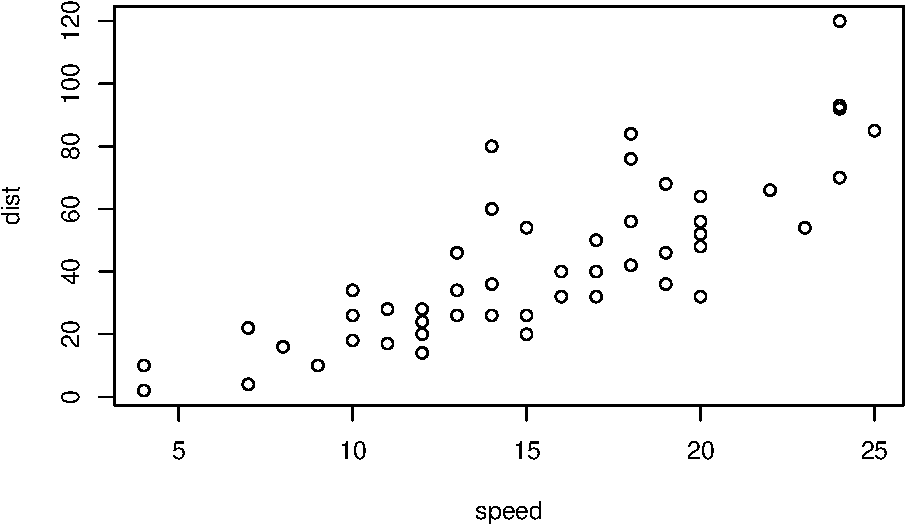
\includegraphics{paper_files/figure-latex/simple-base-plot-1.pdf}
\caption{\label{fig:simple-base-plot}A basic scatterplot of the \texttt{cars} dataset.}
\end{figure}

Figure display size, resolution, file format and many other things can
be controlled by setting the corresponding chunk options. Refer to the
\href{https://yihui.name/knitr/options/\#plots}{plot-related
\texttt{knitr} chunk options} for an overview of all options. In
\texttt{papaja}-documents, by default, all figures as saved as
vectorized PDF and pixel-based PNG files at a resolution of 300 DPI,
which should in most cases be sufficient for print publication. When the
target document format is PDF the vectorized PDF files are included;
when the target document format is DOCX the pixel-based PNG files are
included. The files can be found in the \texttt{mydocument\_files}
folder that is generated when \texttt{mydocument.Rmd} is knitted.

Note, if you define transparent colors in your plots (e.g., when you
defining colors using \texttt{rgb()}), the rendered document will always
display the pixel-based PNG files, regardless of the target document
format. Given the lossless compression in PNG and the decent resolution
of 300 DPI this should not be a problem in print.

\paragraph{\texorpdfstring{\texttt{papaja} plot
functions}{papaja plot functions}}\label{papaja-plot-functions}

Factorial designs are ubiquotous in experimental psychology but
notoriously cumbersome to visualize with R base \texttt{graphics}. That
is why \texttt{papaja} provides a set of functions to facilitate
plotting data from factorial designs.

The functions \texttt{apa\_beeplot()}, \texttt{apa\_lineplot()},
\texttt{apa\_barplot()}, and the generic \texttt{apa\_factorial\_plot()}
are intended to provide a convenient way to obtain a publication-ready
figure while maintaining enough flexibility for customization. The basic
arguments to these functions are all the same, so you only need to learn
one syntax to generate different types of plots. Moreover, it is easy
switch between the different types of plots by changing the name of the
called function.

Consider the following example of a so-called beeswarm plot:





\begin{Shaded}
\begin{Highlighting}[]
\KeywordTok{apa_beeplot}\NormalTok{(}
  \DataTypeTok{data =}\NormalTok{ mixed_data}
\NormalTok{  , }\DataTypeTok{id =} \StringTok{"Subject"}
\NormalTok{  , }\DataTypeTok{dv =} \StringTok{"Recall"}
\NormalTok{  , }\DataTypeTok{factors =} \KeywordTok{c}\NormalTok{(}\StringTok{"Task"}\NormalTok{, }\StringTok{"Valence"}\NormalTok{, }\StringTok{"Dosage"}\NormalTok{)}
\NormalTok{)}
\end{Highlighting}
\end{Shaded}

\begin{figure}
\centering
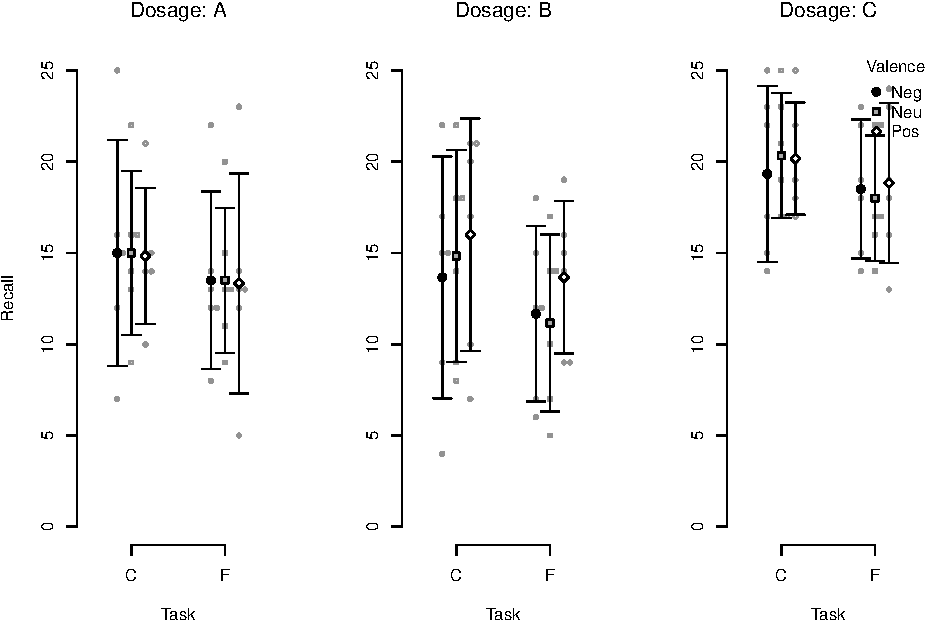
\includegraphics{paper_files/figure-latex/beeswarm2-1.pdf}
\caption{\label{fig:beeswarm2}An example beeswarm plot. Small points represent
individual observations, large points represent condition means, and
error bars represent 95\% confidence intervals.}
\end{figure}

A \texttt{data.frame} that contains the data in long format is passed to
the \texttt{data} argument. The other arguments expect the names of the
columns that contain the subject identifier \texttt{id}, the dependent
variable \texttt{dv}, and the between- or within-subjects
\texttt{factors} of the design. Currently, zero to four factors are
supported.

For each cell of the design, the functions plot

\begin{enumerate}
\def\labelenumi{\arabic{enumi}.}
\tightlist
\item
  central tendency,
\item
  dispersion, and
\item
  names of dependent variable, factors and levels, and optionally a
  legend.
\end{enumerate}

Mesures of central tendency and dispersion default to the mean and 95\%
confidence intervals. However, the arguments \texttt{tendency} and
\texttt{dispersion} can be used to overwrite these defaults and plot
other statistics. For example, to plot within-subject rather than
between-subject confidence intervals you can set
\texttt{dispersion\ =\ within\_subjects\_conf\_int}. If the data
encompass multiple observations per
participant-factor-level-combination, these observations are aggregated.
By default, the condition means are computed but you can specify other
aggregation functions via the \texttt{fun\_aggregate} argument.

The visual elements of the plots can be customized by passing options to
the arguments \texttt{args\_points}, \texttt{args\_error\_bars},
\texttt{args\_legend}, and so on. These arugments take named lists of
arguments that are passed on to the respective \texttt{graphics}
functions, such as \texttt{points()}, \texttt{arrows()}, and
\texttt{legend()}. Consider the following code and the resulting
Figure~\ref{fig:customized-plot} for a customized version of the
previous beeswarm plot.







\begin{figure}
\centering
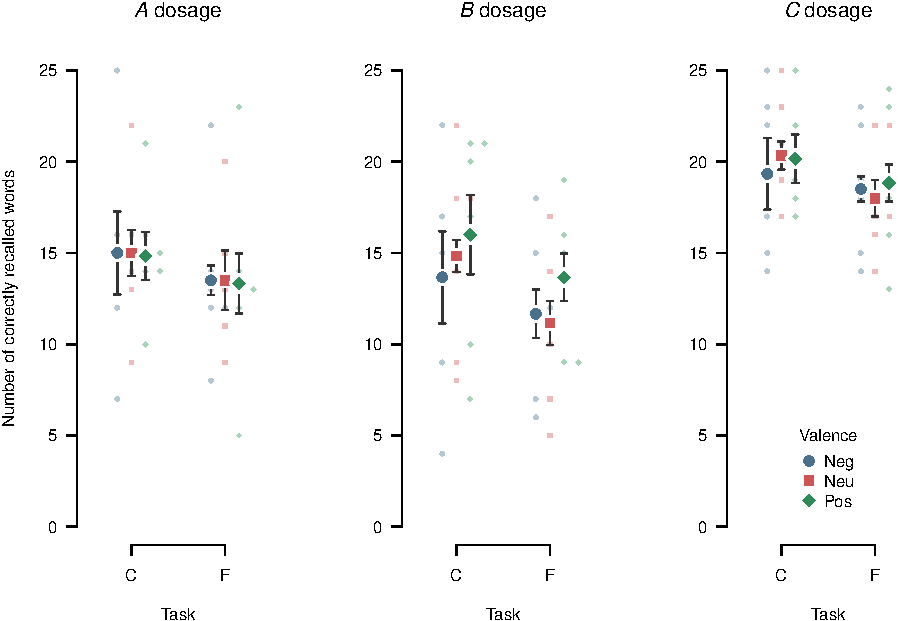
\includegraphics{paper_files/figure-latex/customized-plot-1.pdf}
\caption{\label{fig:customized-plot}A customized beeswarm plot. Note that, by
default, the swarm inherits parameters from the args\_points argument.
Small points represent individual observations, large points represent
means, and error bars represent 95\% within-subjects confidence
intervals.}
\end{figure}

\begin{itemize}
\tightlist
\item
  Utilize variable labels
\end{itemize}

These plot functions also utilize variable labels, with some LaTeX math
support (see \texttt{?latex2exp::TeX})

Custom themes can be set as default as usual and are subsequently
applied to all plots created with \texttt{ggplot()}. \texttt{papaja}
provides a template \texttt{theme\_apa()} that we feel is well suited to
create publication-ready plots. The following example demonstrates how
to set a default theme.

\begin{figure}
\centering
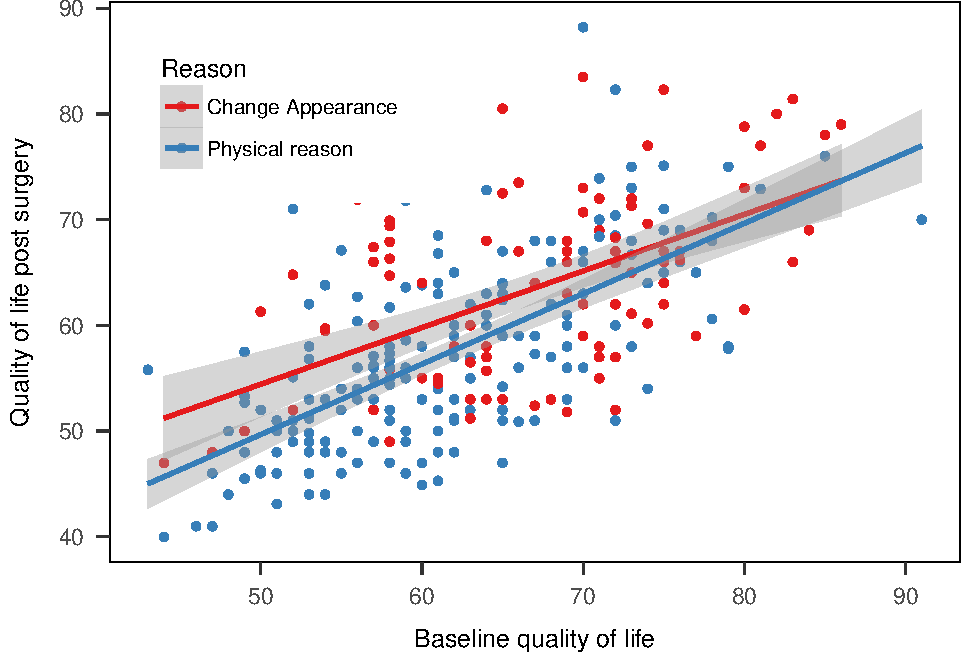
\includegraphics{paper_files/figure-latex/ggplot-1.pdf}
\caption{}
\end{figure}

\hypertarget{tables}{\subsection{Tables}\label{tables}}

For prettier tables, I suggest you try \texttt{apa\_table()}, which
builds on \texttt{knitr}'s \texttt{kable()}.







\begin{Shaded}
\begin{Highlighting}[]
\NormalTok{descriptives <-}\StringTok{ }\NormalTok{mixed_data }\OperatorTok\StringTok{ }\KeywordTok{group_by}\NormalTok{(Dosage) }\OperatorTok
\StringTok{  }\KeywordTok{summarize}\NormalTok{(}
    \DataTypeTok{Mean =} \KeywordTok{mean}\NormalTok{(Recall)}
\NormalTok{    , }\DataTypeTok{Median =} \KeywordTok{median}\NormalTok{(Recall)}
\NormalTok{    , }\DataTypeTok{SD =} \KeywordTok{sd}\NormalTok{(Recall)}
\NormalTok{    , }\DataTypeTok{Min =} \KeywordTok{min}\NormalTok{(Recall)}
\NormalTok{    , }\DataTypeTok{Max =} \KeywordTok{max}\NormalTok{(Recall)}
\NormalTok{  )}
\NormalTok{descriptives[, }\OperatorTok{-}\DecValTok{1}\NormalTok{] <-}\StringTok{ }\KeywordTok{printnum}\NormalTok{(descriptives[, }\OperatorTok{-}\DecValTok{1}\NormalTok{])}

\KeywordTok{apa_table}\NormalTok{(}
\NormalTok{  descriptives}
\NormalTok{  , }\DataTypeTok{caption =} \StringTok{"Descriptive statistics of correct recall by
dosage."}
\NormalTok{  , }\DataTypeTok{note =} \StringTok{"This table was created with
\texttt{apa\_table()}."}
\NormalTok{  , }\DataTypeTok{escape =} \OtherTok{TRUE}
\NormalTok{)}
\end{Highlighting}
\end{Shaded}

Of course popular packages like \texttt{xtable}\footnote{When you use
  \texttt{xtable()}, table captions are
  \href{http://tex.stackexchange.com/questions/42209/centering-tables-in-document-class-apa6}{set
  to the left page margin}.} or \texttt{tables} can also be used to
create tables when knitting PDF documents. These packages, however,
cannot be used when you want to create Microsoft Word documents because
they rely on LaTeX for typesetting. \texttt{apa\_table()} creates tables
that conform to APA guidelines and are correctly rendered in PDF and
Word documents. But don't get too excited. In papaja, table formatting
is somewhat limited for Word documents due to missing functionality in
pandoc (e.g., it is not possible to have cells or headers span across
multiple columns).

As required by the APA guidelines, tables are deferred to the final
pages of the manuscript when creating a PDF. To place tables and figures
in your text instead, set the \texttt{figsintext} parameter in the YAML
header to \texttt{yes} or \texttt{true}, as I have done in this
document. Again, this is not the case in Word documents due to limited
pandoc functionality. The bottom line is, Word documents will be less
polished than PDF. The resulting documents should suffice to enable
collaboration with Wordy colleagues and prepare a journal submission
with limited manual labor.

\subsection{Results from statistical
tests}\label{results-from-statistical-tests}

Output from statistical models and tests needs to be properly formatted
before it can be included in text. For this purpose, we created the
function \texttt{apa\_print()}. Simply drop the results from a
statistical test (e.g.~a \(t\) test or an ANOVA) into
\texttt{apa\_print()}, and you will get an output object (a
\texttt{list}) that contains all you need to report the analysis
according to APA guidelines. \texttt{apa\_print()} currently supports
output objects from a variety of statistical models/tests, including
\(t\) tests, ANOVA, linear regression. For a full list of supported
output objects, see Table \ref{tab:supported-s3-methods}.

A-B

B-H

L-S

S-Z

afex\_aov

BFBayesFactorList*

list

summary\_emm*

anova

BFBayesFactorTop*

lm

summary.glht*

Anova.mlm

emmGrid*

lsmobj*

summary.glm

aov

glht*

summary.Anova.mlm

summary.lm

aovlist

glm

summary.aov

summary.ref.grid*

BFBayesFactor*

htest

summary.aovlist

{* Not fully tested, don't trust blindly!}






\begin{figure}

{\centering 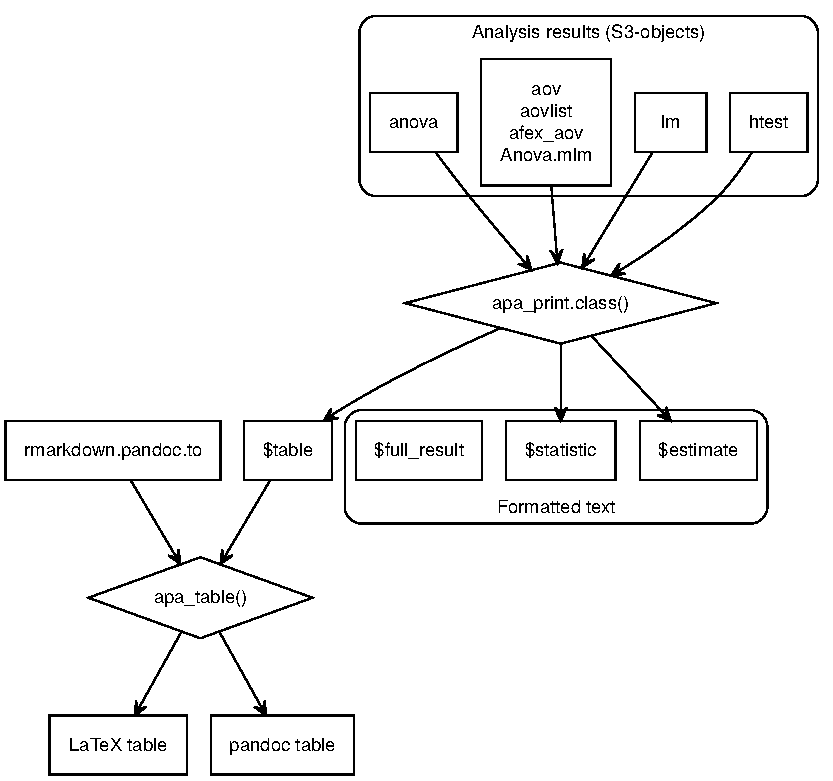
\includegraphics{paper_files/figure-latex/formatting-process-diagram} 

}

\caption{Process diagram illustrating the use of
\texttt{apa\_print()} methods and \texttt{apa\_table()} to format
results from statistical analyses according to APA guidelines. The
formatted text and tables can be reported in a manuscript.}\label{fig:formatting-process-diagram}
\end{figure}

\subsubsection{\texorpdfstring{htest (\emph{t} tests, correlations,
etc.)}{htest (t tests, correlations, etc.)}}\label{htest-t-tests-correlations-etc.}

The results of a \(t\) test (regardless of the exact type of \(t\) test)
are typically stored in an \texttt{htest} object.

\begin{verbatim}
## $estimate
## [1] "$M_d = -3.95$, 95\\% CI $[-4.86$, $-3.04]$"
## 
## $statistic
## [1] "$t(275) = -8.52$, $p < .001$"
## 
## $full_result
## [1] "$M_d = -3.95$, 95\\% CI $[-4.86$, $-3.04]$, $t(275) = -8.52$, $p < .001$"
## 
## $table
## NULL
\end{verbatim}

As you can see, \texttt{apa\_print()} returns a list of four elements:
List element \texttt{estimate} contains the sample estimate of mean
difference; element \texttt{statistic} contains the result of the NHST
with test statistic, \emph{df}s, and \emph{p} value; element
\texttt{full\_result} contains both information combined. The fourth
element, \texttt{table}, contains a table containing test results; while
this is \texttt{NULL} for a \(t\) test, it will be quiet interesting for
ANOVA or linear model results, as you will see in the next subsections.

\subsubsection{lm (linear regression)}\label{lm-linear-regression}

The results of a linear model are stored in an \texttt{lm} object.

Again, \texttt{apa\_print} returns a four-elements list.
\texttt{apa\_lm\$table} contains a complete regression table that can be
passed to \texttt{apa\_table()} to get a full regression table, see
Table @ref(tab:lm-table; remember to set the chunk option
\texttt{results\ =\ "asis"}).

\begin{table}[tbp]
\begin{center}
\begin{threeparttable}
\caption{\label{tab:lm-table}A full regression table.}
\begin{tabular}{lllll}
\toprule
Predictor & \multicolumn{1}{c}{$b$} & \multicolumn{1}{c}{95\% CI} & \multicolumn{1}{c}{$t(273)$} & \multicolumn{1}{c}{$p$}\\
\midrule
Intercept & 18.50 & $[13.10$, $23.91]$ & 6.74 & < .001\\
Base QoL & 0.59 & $[0.50$, $0.67]$ & 13.23 & < .001\\
BDI & 0.17 & $[0.11$, $0.22]$ & 6.08 & < .001\\
\bottomrule
\end{tabular}
\end{threeparttable}
\end{center}
\end{table}

\begin{verbatim}
## [1] "$b = 18.50$, 95\\% CI $[13.10$, $23.91]$"
\end{verbatim}

\begin{quote}
\(b = 18.50\), 95\% CI \([13.10\), \(23.91]\)
\end{quote}

--

\begin{verbatim}
## [1] "$R^2 = .50$, 90\\% CI $[0.42$, $0.57]$, $F(2, 273) = 136.78$, $p < .001$"
\end{verbatim}

\begin{quote}
\(R^2 = .50\), 90\% CI \([0.42\), \(0.57]\), \(F(2, 273) = 136.78\),
\(p < .001\)
\end{quote}

Tables produced by \texttt{apa\_print()} have variable labels

\begin{verbatim}
## A data.frame with 5 labelled columns:
## 
##   predictor estimate                 ci statistic p.value
## 1 Intercept    18.50 $[13.10$, $23.91]$      6.74  < .001
## 2  Base QoL     0.59   $[0.50$, $0.67]$     13.23  < .001
## 3       BDI     0.17   $[0.11$, $0.22]$      6.08  < .001
## 
## predictor: Predictor 
## estimate : $b$ 
## ci       : 95\% CI 
## statistic: $t(273)$ 
## p.value  : $p$
\end{verbatim}

Now, you can report the results of your analyses like so:

\begin{Shaded}
\begin{Highlighting}[]
\KeywordTok{Clinic}\NormalTok{ (}\StringTok{`}\DataTypeTok{r apa_anova$full$Clinic}\StringTok{`}\NormalTok{) and patient gender affected post}\OperatorTok{-}\NormalTok{surgery quality of life, }\StringTok{`}\DataTypeTok{r apa_anova$full$Gender}\StringTok{`}\NormalTok{. However, the effect of gender differed by clinic, }\StringTok{`}\DataTypeTok{r apa_anova$full$Clinic_Gender}\StringTok{`}\NormalTok{.}
\end{Highlighting}
\end{Shaded}

Which will yield the following text:

\begin{quote}
Clinic (\(F(9, 256) = 19.98\), \(\mathit{MSE} = 47.58\), \(p < .001\),
\(\hat{\eta}^2_G = .413\)) and patient gender affected post-surgery
quality of life, \(F(1, 256) = 15.29\), \(\mathit{MSE} = 47.58\),
\(p < .001\), \(\hat{\eta}^2_G = .056\). However, the effect of gender
differed by clinic, \(F(9, 256) = 1.97\), \(\mathit{MSE} = 47.58\),
\(p = .043\), \(\hat{\eta}^2_G = .065\).
\end{quote}

Again, you can easily create a complete ANOVA table by passing
\texttt{recall\_anova\_results\$table} to \texttt{apa\_table()}, see
\autoref{ref:anova}.

\begin{table}[tbp]
\begin{center}
\begin{threeparttable}
\caption{\label{tab:anova-table}A really beautiful ANOVA table.}
\begin{tabular}{lllllll}
\toprule
Effect & \multicolumn{1}{c}{$F$} & \multicolumn{1}{c}{$\mathit{df}_1$} & \multicolumn{1}{c}{$\mathit{df}_2$} & \multicolumn{1}{c}{$\mathit{MSE}$} & \multicolumn{1}{c}{$p$} & \multicolumn{1}{c}{$\hat{\eta}^2_G$}\\
\midrule
Clinic & 19.98 & 9 & 256 & 47.58 & < .001 & .413\\
Gender & 15.29 & 1 & 256 & 47.58 & < .001 & .056\\
Clinic $\times$ Gender & 1.97 & 9 & 256 & 47.58 & .043 & .065\\
\bottomrule
\addlinespace
\end{tabular}
\begin{tablenotes}[para]
\normalsize{\textit{Note.} Note that the column names contain beautiful mathematical copy: This is because the table has variable labels.}
\end{tablenotes}
\end{threeparttable}
\end{center}
\end{table}

\paragraph{glht, lsmeans, ref.grid (post-hoc
tests)}\label{glht-lsmeans-ref.grid-post-hoc-tests}

\ldots{}

\section{Limitations}\label{limitations}

As outlined in \protect\hyperlink{document-compilation}{Document
compilation}, \texttt{papaja} builds on \texttt{pandoc} to render
Markdown into PDF and DOCX documents. Markdown provides good common
basis for these and other document types but the common basis
necessarily limits the degree of control that can be exerted over the
rendered document. For example, there is currently no way to generate
tables with \texttt{pandoc} in which cells span multiple rows or
columns. Similarly, it is not possible to insert page breaks into a
document. Both of these limitations have been raised with the developers
of \texttt{pandoc} (see
\href{https://github.com/jgm/pandoc/issues/1024}{here} and
\href{https://github.com/jgm/pandoc/issues/1934}{here}), but it may take
a while for them to be addressed.

\subsection{PDF documents}\label{pdf-documents}

\texttt{pandoc} builds on LaTeX to render PDF documents. As discussed in
{[}Markdown text formatting{]}, when the R Markdown document contains
LaTeX code it is kept as-is and can be used to exert greater control
over the final result. For example, to create a page break in the
rendered document you can use the LaTeX command
\texttt{\textbackslash{}pagebreak}. Similarly, tables with column
spanners can be created by using the corresponding LaTeX code. Hence,
the limited control offered by \texttt{pandoc} can be compensated by
using LaTeX code and \texttt{papaja} resorts to this approach, for
example, in \texttt{apa\_table()}.

\subsubsection{Customizing the document
preamble}\label{customizing-the-document-preamble}

You can exert further control over your PDF documents by customizing the
LaTeX preamble. Consider the following example: By default, LaTeX
arranges paragraphs and section headings so that they fill the page.
This can sometimes lead to unwanted vertical spacing.

If you prefer white space at the bottom of the page, rather than between
paragraphs, you can overwrite this default behavior by including
\texttt{\textbackslash{}raggedbottom} in the document preamble. To do
so, add the following to the YAML front matter of your document:

\begin{Shaded}
\begin{Highlighting}[]
\FunctionTok{header-includes:}
  \KeywordTok{-}\NormalTok{ \textbackslash{}raggedbottom}
\end{Highlighting}
\end{Shaded}

\subsection{Microsoft Word documents}\label{microsoft-word-documents}

In contrast, there is no simple way to compensate for the limited
control offered by \texttt{pandoc} when rendering Microsoft Word
documents. This is the reason why some of \texttt{papaja}'s features are
only available if the to-be-rendered document is in PDF format, such as
some {[}Rendering options{]} and some features of \texttt{apa\_table()}
(see \protect\hyperlink{tables}{Tables}). More over, rendered documents
in DOCX format require some manual work before they fully comply with
APA guidelines. We, therefore, provide the following checklist of
necessary changes:

Always,

\begin{enumerate}
\def\labelenumi{\arabic{enumi}.}
\tightlist
\item
  add a header line with running head and page number
\end{enumerate}

If necessary,

\begin{enumerate}
\def\labelenumi{\arabic{enumi}.}
\setcounter{enumi}{1}
\tightlist
\item
  position author note at the bottom of page 1
\item
  move figures and tables to the end of the manuscript
\item
  add colon to level 3-headings
\item
  in figure captions,

  \begin{itemize}
  \tightlist
  \item
    add a colon following the figure numbers and italicize(e.g.
    \enquote{\emph{Figure 1}. This is a caption.})
  \end{itemize}
\item
  in tables,

  \begin{itemize}
  \tightlist
  \item
    add horizontal rules above the first and below the last row
  \item
    add midrules
  \end{itemize}
\end{enumerate}

We hope to automated some of these points in the future as the
flexibility of \texttt{pandoc} increases.

\section{Help}\label{help}

\begin{itemize}
\tightlist
\item
  Official documentation: \url{https://crsh.github.io/papaja_man}
\item
  Manuscripts with publicly available R Markdown source files.
\end{itemize}

\begin{verbatim}
## [1] 44
\end{verbatim}

\newpage

\section{References}\label{references}

\begingroup
\setlength{\parindent}{-0.5in} \setlength{\leftskip}{0.5in}

\hypertarget{refs}{}
\hypertarget{ref-american_psychological_association_publication_2010}{}
American Psychological Association. (2010). \emph{Publication Manual of
the American Psychological Association} (6th edition.). Washington, DC:
American Psychological Association.

\hypertarget{ref-asendorpf_recommendations_2013}{}
Asendorpf, J. B., Conner, M., De Fruyt, F., De Houwer, J., Denissen, J.
J. A., Fiedler, K., \ldots{} Wicherts, J. M. (2013). Recommendations for
Increasing Replicability in Psychology. \emph{European Journal of
Personality}, \emph{27}(2), 108--119.
doi:\href{https://doi.org/10.1002/per.1919}{10.1002/per.1919}

\hypertarget{ref-R-papaja}{}
Aust, F., \& Barth, M. (2018). \emph{papaja: Create APA manuscripts with
R Markdown}. Retrieved from \url{https://github.com/crsh/papaja}

\hypertarget{ref-R-Matrix}{}
Bates, D., \& Maechler, M. (2018). \emph{Matrix: Sparse and dense matrix
classes and methods}. Retrieved from
\url{https://CRAN.R-project.org/package=Matrix}

\hypertarget{ref-R-lme4}{}
Bates, D., Mächler, M., Bolker, B., \& Walker, S. (2015). Fitting linear
mixed-effects models using lme4. \emph{Journal of Statistical Software},
\emph{67}(1), 1--48.
doi:\href{https://doi.org/10.18637/jss.v067.i01}{10.18637/jss.v067.i01}

\hypertarget{ref-bem_2011}{}
Bem, D. J. (2011). Feeling the future: Experimental evidence for
anomalous retroactive influences on cognition and affect. \emph{Journal
of Personality and Social Psychology}, \emph{100}(3), 407---425.
doi:\href{https://doi.org/10.1037/a0021524}{10.1037/a0021524}

\hypertarget{ref-cacioppo_social_2015}{}
Cacioppo, J. T., Kaplan, R. M., Krosnick, J. A., Olds, J. L., \& Dean,
H. (2015). \emph{Social, Behavioral, and Economic Sciences Perspectives
on Robust and Reliable Science} (Report of the Subcommittee on
Replicability in Science). Arlington, VA: National Science Foundation.
Retrieved from
\url{http://web.stanford.edu/group/bps/cgi-bin/wordpress/wp-content/uploads/2015/09/NSF-Robust-Research-Workshop-Report.pdf}

\hypertarget{ref-gandrud_reproducible_2013}{}
Gandrud, C. (2013). \emph{Reproducible Research with R and Rstudio}
(Auflage: New.). Boca Raton: Crc Pr Inc.

\hypertarget{ref-R-DiagrammeRsvg}{}
Iannone, R. (2016). \emph{DiagrammeRsvg: Export diagrammer graphviz
graphs as svg}. Retrieved from
\url{https://CRAN.R-project.org/package=DiagrammeRsvg}

\hypertarget{ref-james_1890}{}
James, W. (1890). \emph{The principles of psychology}. Holt: New York.

\hypertarget{ref-R-emmeans}{}
Lenth, R. (2018). \emph{Emmeans: Estimated marginal means, aka
least-squares means}. Retrieved from
\url{https://CRAN.R-project.org/package=emmeans}

\hypertarget{ref-R-bindrcpp}{}
Müller, K. (2018). \emph{Bindrcpp: An 'rcpp' interface to active
bindings}. Retrieved from
\url{https://CRAN.R-project.org/package=bindrcpp}

\hypertarget{ref-R-rsvg}{}
Ooms, J. (2017). \emph{Rsvg: Render svg images into pdf, png,
postscript, or bitmap arrays}. Retrieved from
\url{https://CRAN.R-project.org/package=rsvg}

\hypertarget{ref-R-base}{}
R Core Team. (2018). \emph{R: A language and environment for statistical
computing}. Vienna, Austria: R Foundation for Statistical Computing.
Retrieved from \url{https://www.R-project.org/}

\hypertarget{ref-R-afex}{}
Singmann, H., Bolker, B., Westfall, J., \& Aust, F. (2018). \emph{Afex:
Analysis of factorial experiments}. Retrieved from
\url{https://CRAN.R-project.org/package=afex}

\hypertarget{ref-R-DiagrammeR}{}
Sveidqvist, K., Bostock, M., Pettitt, C., Daines, M., \& Iannone, R.
(2017). \emph{DiagrammeR: Graph/network visualization}. Retrieved from
\url{https://CRAN.R-project.org/package=DiagrammeR}

\hypertarget{ref-R-ggplot2}{}
Wickham, H. (2009). \emph{Ggplot2: Elegant graphics for data analysis}.
Springer-Verlag New York. Retrieved from \url{http://ggplot2.org}

\hypertarget{ref-R-dplyr}{}
Wickham, H., François, R., Henry, L., \& Müller, K. (2018). \emph{Dplyr:
A grammar of data manipulation}. Retrieved from
\url{https://CRAN.R-project.org/package=dplyr}

\hypertarget{ref-R-knitr}{}
Xie, Y. (2015). \emph{Dynamic documents with R and knitr} (2nd ed.).
Boca Raton, Florida: Chapman; Hall/CRC. Retrieved from
\url{https://yihui.name/knitr/}

\endgroup


\end{document}
